

\tikzset{every picture/.style={line width=0.75pt}} %set default line width to 0.75pt        

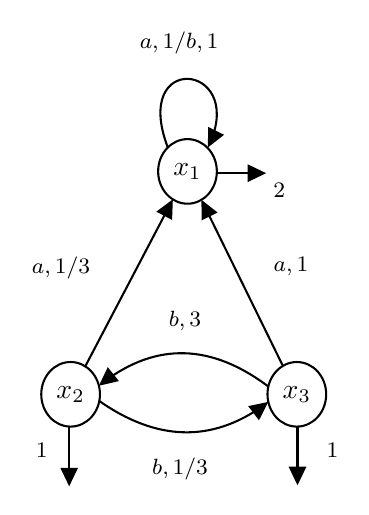
\begin{tikzpicture}[x=0.75pt,y=0.75pt,yscale=-1,xscale=1]
%uncomment if require: \path (0,514); %set diagram left start at 0, and has height of 514

%Curve Lines [id:da7520674866212254] 
\draw    (207.69,98.63) .. controls (223.51,60.79) and (169.45,55.3) .. (187,101.61) ;
\draw [shift={(206.33,101.61)}, rotate = 296.28] [fill={rgb, 255:red, 0; green, 0; blue, 0 }  ][line width=0.08]  [draw opacity=0] (8.93,-4.29) -- (0,0) -- (8.93,4.29) -- cycle    ;
%Straight Lines [id:da36516510379788225] 
\draw    (139.5,236.5) -- (139.5,261.86) ;
\draw [shift={(139.5,264.86)}, rotate = 270] [fill={rgb, 255:red, 0; green, 0; blue, 0 }  ][line width=0.08]  [draw opacity=0] (8.93,-4.29) -- (0,0) -- (8.93,4.29) -- cycle    ;
%Straight Lines [id:da06517112562563687] 
\draw    (249.5,236) -- (249.5,261.36) ;
\draw [shift={(249.5,264.36)}, rotate = 270] [fill={rgb, 255:red, 0; green, 0; blue, 0 }  ][line width=0.08]  [draw opacity=0] (8.93,-4.29) -- (0,0) -- (8.93,4.29) -- cycle    ;
%Straight Lines [id:da05488487732501923] 
\draw    (211,114) -- (231.4,114) ;
\draw [shift={(234.4,114)}, rotate = 180] [fill={rgb, 255:red, 0; green, 0; blue, 0 }  ][line width=0.08]  [draw opacity=0] (8.93,-4.29) -- (0,0) -- (8.93,4.29) -- cycle    ;

% Text Node
\draw    (196.5, 113.15) circle [x radius= 14.14, y radius= 15.56]   ;
\draw (196.5,113.15) node  [font=\normalsize]  {$x_{1}$};
% Text Node
\draw    (140.18, 220.54) circle [x radius= 14.14, y radius= 15.56]   ;
\draw (140.18,220.54) node  [font=\normalsize]  {$x_{2}$};
% Text Node
\draw    (249.18, 220.54) circle [x radius= 14.14, y radius= 15.56]   ;
\draw (249.18,220.54) node  [font=\normalsize]  {$x_{3}$};
% Text Node
\draw (178,249.9) node [anchor=north west][inner sep=0.75pt]  [font=\footnotesize]  {$b,1/3$};
% Text Node
\draw (186,178.9) node [anchor=north west][inner sep=0.75pt]  [font=\footnotesize]  {$b,3$};
% Text Node
\draw (236.5,152.9) node [anchor=north west][inner sep=0.75pt]  [font=\footnotesize]  {$a,1$};
% Text Node
\draw (172,44.4) node [anchor=north west][inner sep=0.75pt]  [font=\footnotesize]  {$a,1/b,1$};
% Text Node
\draw (120,152.9) node [anchor=north west][inner sep=0.75pt]  [font=\footnotesize]  {$a,1/3$};
% Text Node
\draw (122,242.65) node [anchor=north west][inner sep=0.75pt]  [font=\footnotesize]  {$1$};
% Text Node
\draw (262,242.65) node [anchor=north west][inner sep=0.75pt]  [font=\footnotesize]  {$1$};
% Text Node
\draw (236.4,117.4) node [anchor=north west][inner sep=0.75pt]  [font=\footnotesize]  {$2$};
% Connection
\draw    (154.02,223.76) .. controls (181.71,243.14) and (208.08,243.86) .. (233.12,225.93) ;
\draw [shift={(235.43,224.21)}, rotate = 502.59] [fill={rgb, 255:red, 0; green, 0; blue, 0 }  ][line width=0.08]  [draw opacity=0] (8.93,-4.29) -- (0,0) -- (8.93,4.29) -- cycle    ;
% Connection
\draw    (235.45,216.79) .. controls (208,196.14) and (181.57,195.41) .. (156.17,214.59) ;
\draw [shift={(153.82,216.42)}, rotate = 321.14] [fill={rgb, 255:red, 0; green, 0; blue, 0 }  ][line width=0.08]  [draw opacity=0] (8.93,-4.29) -- (0,0) -- (8.93,4.29) -- cycle    ;
% Connection
\draw    (147.25,207.06) -- (188.04,129.28) ;
\draw [shift={(189.43,126.63)}, rotate = 477.67] [fill={rgb, 255:red, 0; green, 0; blue, 0 }  ][line width=0.08]  [draw opacity=0] (8.93,-4.29) -- (0,0) -- (8.93,4.29) -- cycle    ;
% Connection
\draw    (242.46,206.85) -- (204.54,129.53) ;
\draw [shift={(203.22,126.84)}, rotate = 423.87] [fill={rgb, 255:red, 0; green, 0; blue, 0 }  ][line width=0.08]  [draw opacity=0] (8.93,-4.29) -- (0,0) -- (8.93,4.29) -- cycle    ;

\end{tikzpicture}
